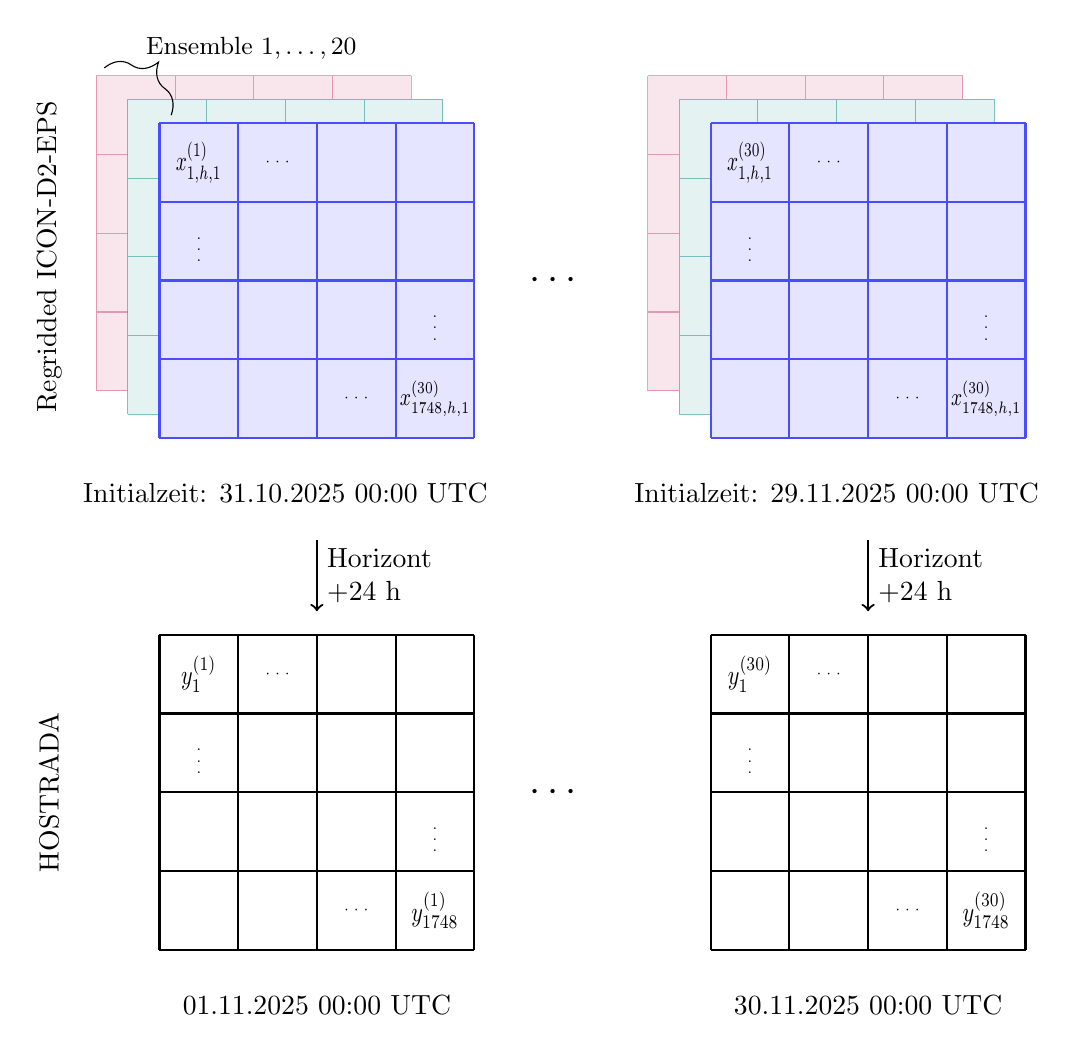
\begin{tikzpicture}%[scale=0.5,, transform shape]
\def\N{4}
\def\dy{-6.5} % vertikaler Versatz der Verifikationszeile nach unten
\def\dx{7} %horizontaler versatz der gitter

% =========================================================
% Zeilenbeschriftung links: Ensemble-Reihe
% =========================================================
\node[rotate=90] at (-1.4,2.3) {Regridded ICON-D2-EPS};
% =========================================================
% ENSEMBLE-REIHE (oben)
% =========================================================
% --- Ensemble-Grafik 1 ---
\begin{scope}[shift={(0,0)}]
% Ensemble 3 (hinten)
\begin{scope}[shift={(-0.8,0.6)}]
    \fill[purple!10] (0,0) rectangle (\N,\N);
    \draw[purple!70, opacity=0.5] (0,0) grid (\N,\N);
\end{scope}
% Ensemble 2 (mittig)
\begin{scope}[shift={(-0.4,0.3)}]
    \fill[teal!10] (0,0) rectangle (\N,\N);
    \draw[teal!70, opacity=0.7] (0,0) grid (\N,\N);
\end{scope}
% Ensemble 1 (vorne)
\fill[blue!10] (0,0) rectangle (\N,\N);
\draw[blue!70, thick] (0,0) grid (\N,\N);


% Werte
\node  at (0.5,\N-0.5) { \scalebox{0.7}[1]{$x_{1,h,1}^{(1)}$}};
\node[font=\small] at (\N-0.5,0.5) {\scalebox{0.77}[1]{$x_{1748,h,1}^{(30)}$}};
% rechts daneben
\node[font=\tiny] at (1.5,\N-0.5) {$\cdots$};
% darunter
\node[font=\tiny] at (0.5,\N-1.5) {$\vdots$};
% links neben B
\node[font=\tiny] at (\N-1.5,0.5) {$\cdots$};
% oberhalb von B
\node[font=\tiny] at (\N-0.5,1.5) {$\vdots$};


% Klammer
\draw[decorate, decoration={brace, amplitude=13pt}]
(-0.7,\N+.7) -- (0.15,\N+.1)
node[near end, yshift=20pt,xshift=35pt,font=\small]
{Ensemble $1, \ldots, 20$};
\node at (1.6,-0.7) {Initialzeit: 31.10.2025 00:00 UTC};
\end{scope}

\node at (5,2) {\Large $\cdots$};

% --- Ensemble-Grafik 2 ---
\begin{scope}[shift={(\dx,0)}]
\begin{scope}[shift={(-0.8,0.6)}]
    \fill[purple!10] (0,0) rectangle (\N,\N);
    \draw[purple!70, opacity=0.5] (0,0) grid (\N,\N);
\end{scope}
\begin{scope}[shift={(-0.4,0.3)}]
    \fill[teal!10] (0,0) rectangle (\N,\N);
    \draw[teal!70, opacity=0.7] (0,0) grid (\N,\N);
\end{scope}
\fill[blue!10] (0,0) rectangle (\N,\N);
\draw[blue!70, thick] (0,0) grid (\N,\N);
\node at (1.6,-0.7) {Initialzeit: 29.11.2025 00:00 UTC};


\node  at (0.5,\N-0.5) { \scalebox{0.7}[1]{$x_{1,h,1}^{(30)}$}};
\node[font=\small] at (\N-0.5,0.5) {\scalebox{0.77}[1]{$x_{1748,h,1}^{(30)}$}};
% rechts daneben
\node[font=\tiny] at (1.5,\N-0.5) {$\cdots$};
% darunter
\node[font=\tiny] at (0.5,\N-1.5) {$\vdots$};
% links neben B
\node[font=\tiny] at (\N-1.5,0.5) {$\cdots$};
% oberhalb von B
\node[font=\tiny] at (\N-0.5,1.5) {$\vdots$};
\end{scope}

% =========================================================
% Pfeil: Vorhersagehorizont (nach unten, innerhalb der Spalte)
% =========================================================
\draw[->, thick]
    (2,-1.3) -- node[right, align=left] {Horizont\\ +24 h} (2,\dy+\N+0.3);
\draw[->, thick]
    (2+\dx,-1.3) -- node[right, align=left] {Horizont\\ +24 h} (2+\dx,\dy+\N+0.3);
% =========================================================
% Zeilenbeschriftung links: Verifikations-Reihe
% =========================================================
\node[rotate=90] at (-1.4,\dy+2) {HOSTRADA};

% =========================================================
% VERIFIKATIONS-REIHE (unten)
% =========================================================
\begin{scope}[shift={(0,\dy)}]
\draw[black, thick] (0,0) grid (\N,\N);
\node at (2,-0.7) {01.11.2025 00:00 UTC};

\node  at (0.5,\N-0.5) { \scalebox{0.8}[1]{$y_{1}^{(1)}$}};
\node at (\N-0.5,0.5) {\scalebox{0.8}[1]{$y_{1748}^{(1)}$}};
\node[font=\tiny] at (1.5,\N-0.5) {$\cdots$};
\node[font=\tiny] at (0.5,\N-1.5) {$\vdots$};
\node[font=\tiny] at (\N-1.5,0.5) {$\cdots$};
\node[font=\tiny] at (\N-0.5,1.5) {$\vdots$};

\end{scope}

\node at (5,\dy+2) {\Large $\cdots$};


\begin{scope}[shift={(7,\dy)}]
\draw[black, thick] (0,0) grid (\N,\N);
\node at (2,-0.7) {30.11.2025 00:00 UTC};
\node  at (0.5,\N-0.5) { \scalebox{0.8}[1]{$y_{1}^{(30)}$}};
\node at (\N-0.5,0.5) {\scalebox{0.8}[1]{$y_{1748}^{(30)}$}};
\node[font=\tiny] at (1.5,\N-0.5) {$\cdots$};
\node[font=\tiny] at (0.5,\N-1.5) {$\vdots$};
\node[font=\tiny] at (\N-1.5,0.5) {$\cdots$};
\node[font=\tiny] at (\N-0.5,1.5) {$\vdots$};
\end{scope}

\end{tikzpicture}